\chapter{Grenzen kontextfreier Sprachen$^*$} 
In diesem Kapitel diskutieren wir die Grenzen kontextfreier Sprachen und leiten dazu das
sogenannte ``\emph{gro{\ss}e Pumping-Lemma}'' her, mit dessen Hilfe wir beispielsweise zeigen
k\"onnen, dass die Sprache $L_{\mbox{\scriptsize \textsl{square}}}$, die durch
\\[0.2cm]
\hspace*{1.3cm} $L_{\mbox{\scriptsize \textsl{square}}} = \bigl\{ ww \mid w \in \Sigma^*\bigr\}$
\\[0.2cm]
definiert wird, f\"ur das Alphabet $\Sigma =\{\texttt{a}, \texttt{b}\}$ keine kontextfreie Sprache
ist.  Bevor wir das Pumping-Lemma f\"ur kontextfreie Sprachen beweisen, zeigen wir, wie sich nutzlose
Symbole aus einer Grammatik entfernen lassen. 

\section{Beseitigung nutzloser Symbole$^*$}
In diesem Abschnitt zeigen wir, wie wir nutzlose Symbole aus einer kontextfreien Grammatik entfernen
k\"onnen. Ist $G = \langle V, T, R, S \rangle$ eine kontextfreie Grammatik, so nennen wir
eine syntaktische Variable $A \in V$ \emph{n\"utzlich}, wenn es Strings $w \in T^*$ und
$\alpha,\beta \in (V \cup T)^*$ gibt, so dass  
\\[0.2cm]
\hspace*{1.3cm}
$S \Rightarrow^* \alpha A \beta \Rightarrow^* w$
\\[0.2cm]
gilt.  Eine syntaktische Variable ist also genau dann n\"utzlich, wenn diese Variable in der Herleitung
eines Wortes $w \in L(G)$ verwendet werden kann.  Analog hei{\ss}t
ein Terminal $t \in T$ \emph{n\"utzlich}, wenn es W\"orter $w_1, w_2 \in T^*$ gibt, so dass
\\[0.2cm]
\hspace*{1.3cm}
$S \Rightarrow^* w_1 t w_2$
\\[0.2cm]
gilt.  Ein Terminal $t$ ist also genau dann n\"utzlich, wenn es in einem Wort  $w \in L(G)$
auftritt.  Variablen und Terminale, die nicht n\"utzlich sind, bezeichnen wir als
\emph{nutzlose Symbole}.

Die Erkennung nutzloser Symbole ist eine \"Uberpr\"ufung, die in manchen Parser-Generatoren
(beispielsweise in \textsl{Bison}\footnote{
\textsl{Bison} ist ein Parser-Generator f\"ur die Sprache \texttt{C}.}) 
eingebaut ist, weil das Auftreten nutzloser Symbole oft
einen Hinweis darauf gibt, dass die Grammatik nicht die Sprache beschreibt, die intendiert ist.  
Insofern ist die jetzt vorgestellte Technik auch von praktischem Interesse.
Wir beginnen mit zwei Definitionen.

\begin{Definition}[erzeugende Variable] \lb
Eine syntaktische Variable $A \in V$ einer Grammatik $G = \langle V, T, R, S \rangle$ 
ist eine \emph{erzeugende} Variable, wenn es ein Wort $w \in T^*$ gibt, so dass
\\[0.2cm]
\hspace*{1.3cm}
$A \Rightarrow^* w$
\\[0.2cm]
gilt, aus einer erzeugende Variable l\"asst sich also immer mindestens ein Wort aus $T^*$ herleiten. 
Die Notation $A \Rightarrow^* w$ dr\"uckt aus, dass das Wort $w$ aus der Variablen $A$ in endlich vielen
Schritten abgeleitet werden kann.
\qed 
\end{Definition}

\noindent
Offenbar ist eine syntaktische Variable, die nicht erzeugend ist, nutzlos.  Die Menge aller
erzeugenden Variablen einer Grammatik $G$  kann mit Hilfe der folgenden induktiven Definition
gefunden werden.
\begin{enumerate}
\item Enth\"alt die Grammatik $G = \langle V, T, R, S \rangle$ eine Regel der Form
      \\[0.2cm]
      \hspace*{1.3cm}
       $A \rightarrow w$ \quad mit $w \in T^*$, 
      \\[0.2cm]
      so ist die Variable $A$ offenbar erzeugend.
\item Enth\"alt die Grammatik $G = \langle V, T, R, S \rangle$ eine Regel der Form
      \\[0.2cm]
      \hspace*{1.3cm}
       $A \rightarrow \alpha$ 
      \\[0.2cm]
      und sind alle syntaktischen Variablen, die in dem Wort $\alpha$ auftreten, bereits
      als erzeugende Variablen 
      erkannt, so ist auch die syntaktische Variable $A$ erzeugend.
\end{enumerate}

\example
Es sei $G = \langle \{S, A, B, C\}, \{ \texttt{x} \}, R, S \rangle$ und die Menge der Regeln $R$
sei wie folgt gegeben:
\begin{eqnarray*}
  S & \rightarrow & A B C \mid A,           \\
  A & \rightarrow & A A \mid \texttt{x},    \\
  B & \rightarrow & A C,                    \\
  C & \rightarrow & B A.                    
\end{eqnarray*}
Aufgrund der Regel
\\[0.2cm]
\hspace*{1.3cm}
$A \rightarrow \texttt{x}$
\\[0.2cm]
ist zun\"achst $A$ erzeugend.  Aufgrund der Regel
\\[0.2cm]
\hspace*{1.3cm}
$S \rightarrow A$
\\[0.2cm]
ist dann auch $S$ erzeugend.  Die Variablen $B$ und $C$ sind hingegen nicht erzeugend und damit sicher
nutzlos.  \qed
\vspace*{0.2cm}


\noindent
Ist $G = \langle V, T, R, S \rangle$ eine Grammatik und ist $E$ die Menge der erzeugenden Variablen,
so k\"onnen wir alle Variablen, die nicht erzeugend sind, einfach weglassen.  Zus\"atzlich m\"ussen wir
nat\"urlich auch die Regeln weglassen, in denen Variablen auftreten, die nicht erzeugend sind.  Dabei
\"andert sich die von der Grammatik $G$ erzeugte Sprache offenbar nicht.

Eine Variable kann gleichzeitig erzeugend und trotzdem nutzlos sein.  Als einfaches
Beispiel betrachten wir die Grammatik  $G = \langle \{S, A, B \}, \{ \texttt{x}, \texttt{y} \}, R, S \rangle$, deren Regeln durch
\begin{eqnarray*}
  S & \rightarrow & A \texttt{y},           \\
  A & \rightarrow & A A \mid \texttt{x} \quad \mbox{und}    \\
  B & \rightarrow & A \texttt{y} 
\end{eqnarray*}
gegeben sind.  Die erzeugenden Variable sind in diesem Falle $A$, $B$ und $S$.  Die Variable
$B$ ist trotzdem nutzlos, denn von $S$ aus ist diese Variable gar nicht \emph{erreichbar}.
Formal definieren wir f\"ur eine Grammatik $G = \langle V, T, R, S \rangle$ eine syntaktische Variable $X$ als
\emph{erreichbar}, wenn es W\"orter $\alpha, \beta \in (V \cup T)^*$ gibt, so dass 
\\[0.2cm]
\hspace*{1.3cm}
$S \Rightarrow^* \alpha X \beta$
\\[0.2cm]
gilt. F\"ur eine gegebene Grammatik $G$  l\"asst sich die Menge der Variablen, die erreichbar
sind, mit dem folgenden 
induktiven Algorithmus berechnen.
\begin{enumerate}
\item Das Start-Symbol $S$ ist erreichbar.
\item Enth\"alt die Grammatik $G$ eine Regel der Form
      \\[0.2cm]
      \hspace*{1.3cm}
      $X \rightarrow \alpha$
      \\[0.2cm]
      und ist $X$ erreichbar, so sind auch alle Variablen, die in $\alpha$ auftreten, erreichbar.
\end{enumerate}
Offenbar sind Variablen, die nicht erreichbar sind, nutzlos und wir k\"onnen diese Variablen, sowie alle
Regeln, in denen diese Variablen auftreten, weglassen, ohne dass sich dabei die Sprache \"andert.
Damit haben wir jetzt ein Verfahren, um aus einer Grammatik alle nutzlosen Variablen zu entfernen.
\begin{enumerate}
\item Zun\"achst entfernen wir alle Variablen, die nicht erzeugend sind.
\item Anschlie{\ss}end entfernen wir alle Variablen, die nicht erreichbar sind.
\end{enumerate}
Es ist wichtig zu verstehen, dass die Reihenfolge der obigen Regeln nicht umgedreht werden darf.
Dazu betrachten wir die Grammatik  $G = \langle \{S, A, B, C\}, \{ \texttt{x}, \texttt{y} \}, R, S \rangle$, deren Regeln durch
\begin{eqnarray*}
  S & \rightarrow & B C \mid A,             \\
  A & \rightarrow & A A \mid \texttt{x},    \\
  B & \rightarrow & \texttt{y} \hspace*{1.3cm} \mbox{und} \\
  C & \rightarrow & C C 
\end{eqnarray*}
gegeben sind.  Die beiden Regeln
\\[0.2cm]
\hspace*{1.3cm}
$S \rightarrow BC$ \quad und \quad $S \rightarrow A$
\\[0.2cm]
zeigen, dass alle Variablen erreichbar sind.  Weiter sehen wir, dass die Variablen $A$, $B$ und $S$
erzeugend sind, denn es gilt
\\[0.2cm]
\hspace*{1.3cm}
$A \Rightarrow^* \texttt{x}$, \quad
$S \Rightarrow^* \texttt{x}$  \quad und \quad
$B \Rightarrow^* \texttt{y}$.
\\[0.2cm]
Damit sieht es zun\"achst so aus, als ob nur $C$ nutzlos ist.  Das stimmt aber nicht, auch die Variable
$B$ ist nutzlos, denn wenn wir die Variable $C$ aus der Grammatik entfernen, dann wird auch die Regel
\\[0.2cm]
\hspace*{1.3cm}
$S \rightarrow BC$
\\[0.2cm]
entfernt und damit ist dann $B$ nicht mehr erreichbar und somit ebenfalls nutzlos.

\remark
An dieser Stelle k\"onnen wir uns fragen, warum es funktioniert, wenn wir erst alle Variablen 
entfernen, die nicht erzeugend sind und anschlie{\ss}end dann die nicht erreichbaren Variablen entfernen.
Der Grund ist, dass eine Variable $B$, die nicht erreichbar ist, niemals von einer
anderen Variablen $A$, die erreichbar ist, ben\"otigt wird um ein Wort $w\in T^*$ abzuleiten, denn
wenn die Variable $B$ in der Ableitung
\\[0.2cm]
\hspace*{1.3cm}
$A \Rightarrow^* w$
\\[0.2cm]
auftritt, dann folgt aus der Erreichbarkeit von $A$ auch die Erreichbarkeit von $B$.
Wenn also eine Variable $A$ gleichzeitig erreichbar und  erzeugend ist und wir andererseits eine Variable
$B$ als nicht erreichbar erkannt haben, dann kann $B$ getrost entfernt werden, denn das kann 
an der Tatsache, dass $A$ erzeugend ist, nichts \"andern. \eox

\remark
Der nachfolgende Beweis des Pumping-Lemmas ist logisch von der Beseitigung der nutzlosen
Symbole unabh\"angig.  Das war in einer fr\"uheren Version dieses Skriptes anders, denn bei
dem damals verwendeten Beweis war es notwendig, die Grammatik vorher in
\emph{Chomsky-Normal-Form} zu transformieren.  Die Beseitigung der nutzlosen
Symbole ist ein Teil dieser Transformation.  Der gleich folgende Beweis setzt nicht mehr
voraus, dass die Grammatik in Chomsky-Normal-Form vorliegt.  Da die Technik der
Beseitigung nutzloser Symbole aber auch einen praktischen Wert hat, habe ich diesen
Abschnitt trotzdem beibehalten. 

\section{Parse-B\"aume als Listen}
Zum Beweis des Pumping-Lemmas f\"ur kontextfreie Sprachen ben\"otigen wir eine
Absch\"atzung, bei der wir die L\"ange eines Wortes $w$ aus einer kontextfreien Sprache $L(G)$ 
mit der H\"ohe des Parse-Baums f\"ur $W$ in Verbindung bringen.  Es zeigt sich, dass es zum Nachweis dieser
Absch\"atzung hilfreich ist, wenn wir einen Parse-Baum als Liste aller Pfade des Parse-Baums auffassen.
Die Idee wird am ehesten anhand eines Beispiels klar.  Abbildung
\ref{fig:parse-tree.dot2} auf Seite \pageref{fig:parse-tree.dot2}
zeigt einen Parse-Baum f\"ur den String ``\texttt{2*3+4}'', der mit Hilfe der in Abbildung
\ref{fig:ArithExpr} gezeigten Grammatik erstellt wurde. 

\begin{figure}[htbp]
  \begin{center}    
  \framebox{
  \framebox{
  \begin{minipage}[t]{8cm}
  \begin{eqnarray*}
  \textsl{expr}    & \rightarrow & \;\textsl{expr} \quoted{+} \textsl{product}  \\
                   & \mid        & \;\textsl{expr} \quoted{-} \textsl{product}  \\
                   & \mid        & \;\textsl{product}                           \\[0.2cm]
  \textsl{product} & \rightarrow & \;\textsl{product} \quoted{*} \textsl{factor}\\
                   & \mid        & \;\textsl{product} \quoted{/} \textsl{factor}\\
                   & \mid        & \;\textsl{factor}                            \\[0.2cm]
  \textsl{factor}  & \rightarrow &   \quoted{(} \textsl{expr} \quoted{)}        \\
                   & \mid        &   \quoted{2} \mid \quoted{3} \mid \quoted{4} 
  \end{eqnarray*}
  \vspace*{-0.5cm}
  \end{minipage}}}
  \end{center}
  \caption{Grammatik f\"ur arithmetische Ausdr\"ucke.}
  \label{fig:ArithExpr}
\end{figure}
\vspace*{0.3cm}


\begin{figure}[!ht]
  \centering
      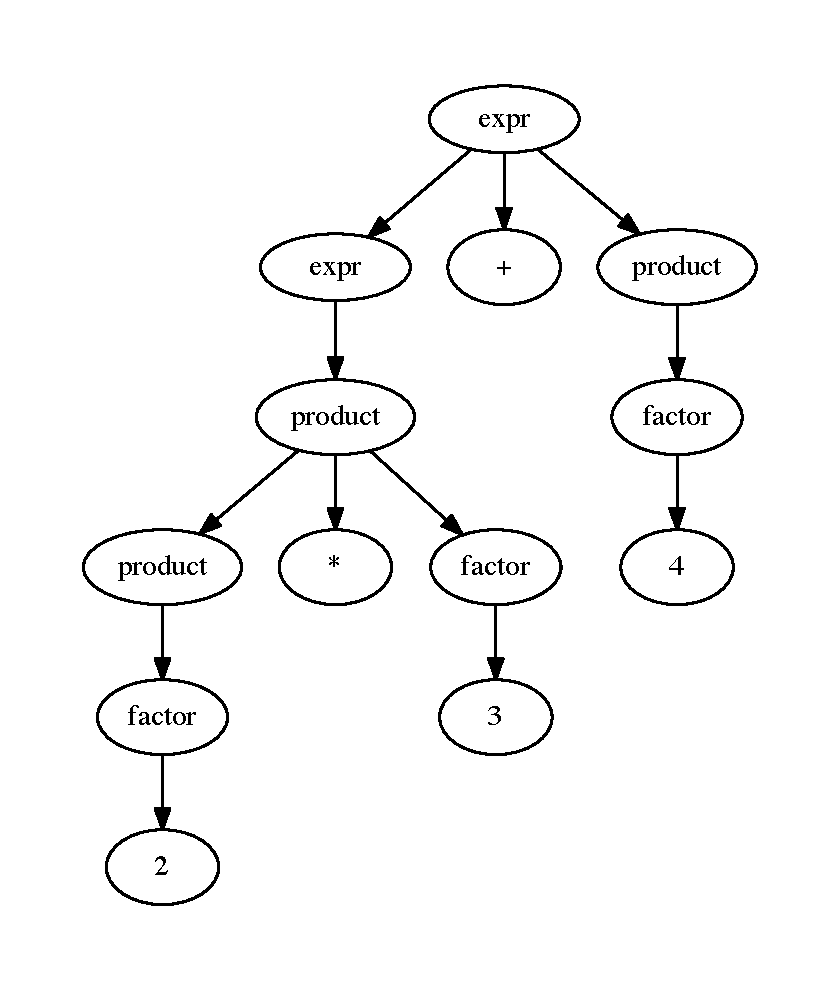
\epsfig{file=Abbildungen/parse-tree.eps, scale=0.6}
  \caption{Ein Parse-Baum f\"ur den String ``\texttt{2*3+4}''.}
  \label{fig:parse-tree.dot2}
\end{figure}

Fassen wir diesen Parse-Baum als Liste seiner
Zweige auf, wobei jeder Zweig eine Liste von Grammatik-Symbolen ist, so erhalten wir die folgende Liste:
\\[0.2cm]
\hspace*{1.3cm}
$
\begin{array}[b]{rl}
  \bigl[ 
 & [ \textsl{expr}, \textsl{expr}, \textsl{product}, \textsl{product}, \textsl{factor}, \quoted{2} ],
   \\[0.1cm] 
 & [ \textsl{expr}, \textsl{expr}, \textsl{product}, \quoted{*} ],
   \\[0.1cm] 
 & [ \textsl{expr}, \textsl{expr}, \textsl{product}, \textsl{factor}, \quoted{3} ],
   \\[0.1cm] 
 & [ \textsl{expr}, \quoted{+} ],
   \\[0.1cm] 
 & [ \textsl{expr}, \textsl{product}, \textsl{factor}, \quoted{4} ]
   \\[0.1cm] 
  \bigr]. 
\end{array}
$ \eox
\pagebreak

\noindent
Die nun folgende Definition der Funktion $\textsl{parseTree}()$ formalisiert die
Berechnung des Parse-Baums.

\begin{Definition}[\textsl{parseTree}] \lb
Ist $G = \langle V, T, R, S \rangle$ eine kontextfreie Grammatik, ist $w \in T^*$, $A \in V$ und  gibt es eine Ableitung
\[ A \Rightarrow^* w,  \]
so definieren wir $\textsl{parseTree}(A \Rightarrow^* w)$ induktiv als Liste von Listen:
\begin{enumerate}
\item Falls $(A \rightarrow t_1t_2 \cdots t_m)\in R$ mit $A \in V$ und $t_1 \cdots t_m = w$ ist,
      so setzen wir
      \\[0.2cm]
      \hspace*{1.3cm}
      $\textsl{parseTree}(A \Rightarrow^* w) = \bigl[\, [A, t_1],\,  [A, t_2],\,\cdots,\,  [A, t_m]\, \bigr]$.  
\item Falls $(A \rightarrow \varepsilon)\in R$ mit $A \in V$ und $w = \varepsilon$ ist, so setzen wir
      \\[0.2cm]
      \hspace*{1.3cm}
      $\textsl{parseTree}(A \Rightarrow^* w) = \bigl[\, [A, \varepsilon]\, \bigr]$.  
\item Falls  $A \Rightarrow^* w$ gilt, weil
      \\[0.2cm]
      \hspace*{1.3cm}
      $ (A \rightarrow B_1B_2 \cdots B_m) \in R, \quad 
         B_i \Rightarrow^* w_i\; \mbox{f\"ur alle $i=1,\cdots,m$} \quad
         \mbox{und} \; w = w_1w_2 \cdots w_m
      $
      \\[0.2cm]
      gilt, so definieren wir (unter Benutzung der \textsc{SetlX}-Notation f\"ur die Definition von Listen)
      \\[0.2cm]
      \hspace*{1.3cm}
      $ 
        \textsl{parseTree}(A \Rightarrow^*w)  =
        \bigl[\; [A] + l \,:\,
                 i \in [1, \cdots, m ],\, l \in \textsl{parseTree}(B_i \Rightarrow^* w_i) \;
        \bigr]
      $.
      \\[0.2cm]
      Damit diese Definition auch tats\"achlich alle F\"alle abdeckt, m\"ussen wir noch den Fall
      diskutieren, dass  eines der Symbole $B_i$ ein Terminal ist: In diesem Fall setzen wir
      \\[0.2cm]
      \hspace*{1.3cm}
      $\textsl{parseTree}(B_i \Rightarrow^* B_i) := \bigl[ [B_i] \bigr]$.
\end{enumerate}
\end{Definition}

Wir definieren die \emph{Breite} $b$ einer Grammatik als die gr\"o{\ss}te Anzahl von Symbolen, die 
auf der rechten Seite einer Grammatik-Regel der Form
\\[0.2cm]
\hspace*{1.3cm}
$A \rightarrow \alpha$
\\[0.2cm]
auftreten.  

\begin{Lemma}[Beschr\"anktheits-Lemma] \label{lemma:length}
  Die Grammatik $G = \langle V, T, R, S \rangle$ habe die Breite $b$.  Ferner gelte
  \\[0.2cm]
  \hspace*{1.3cm}
  $A \Rightarrow^* w$
  \\[0.2cm]
  f\"ur eine syntaktische Variable $A \in V$ und ein Wort $w \in T^*$.  Falls $n$ die L\"ange der l\"angsten Liste in
  \[ \textsl{parseTree}(A \Rightarrow^* w) \]
  ist, so gilt f\"ur die L\"ange des Wortes $w$ die Absch\"atzung
  \\[0.2cm]
  \hspace*{1.3cm}
  $|w| \leq b^{n-1}$.  
\end{Lemma}

\noindent
\textbf{Beweis}: Wir f\"uhren den Beweis durch Induktion nach der L\"ange $n$ der l\"angsten
Liste in $\textsl{parseTree}(A \Rightarrow^* w)$.
\begin{enumerate}
\item[I.A.] $n=2$:  Wenn alle Listen in $\textsl{parseTree}(A \Rightarrow^* w)$ 
            nur zwei Elemente haben, dann besteht die Ableitung aus genau einem Schritt
            und daher muss es eine Regel der Form 
            \\[0.2cm]
            \hspace*{1.3cm}
            $A \rightarrow t_1t_2 \cdots t_m$ \quad mit $w = t_1t_2 \cdots t_m$ und $t_i \in T$
            f\"ur alle $i=1,\cdots,m$
            \\[0.2cm]
            in der Grammatik $G$ geben.  Es gilt dann
            \[ \textsl{parseTree}(A \Rightarrow^* w) = 
               \bigl[\, [A,t_1],\, [A,t_2],\, \cdots,\; [A,t_m]\, \bigr].\, 
            \]
            Daraus folgt
            \\[0.2cm]
            \hspace*{1.3cm}
            $|w| = |t_1t_2 \cdots t_m| = m \leq b = b^{1} = b^{2-1}$,
            \\[0.2cm]
            wobei die Ungleichung $m \leq b$ aus der Tatsache folgt, dass die L\"ange der Regeln der Grammatik
            $G$ durch die Breite $b$ beschr\"ankt ist.
\item[I.S.] $n \mapsto n+1$: Da die Ableitung nun aus mehr als einem Schritt besteht, hat die Ableitung die Form
            \\[0.2cm]
            \hspace*{1.3cm}
            $A \Rightarrow B_1 B_2 \cdots B_m \Rightarrow^* w_1 w_2 \cdots w_m = w$.
            \\[0.2cm]
            Au{\ss}erdem haben dann die Listen in
            \[ 
               \textsl{parseTree}(B_i \Rightarrow^* w_i) 
            \]
            f\"ur alle $i=1,\cdots,m$ h\"ochstens die L\"ange $n$.
            Nach Induktions-Voraussetzung wissen wir also, dass
            \\[0.2cm]
            \hspace*{1.3cm}
            $|w_i| \leq b^{n-1}$ \quad f\"ur alle $i=1,\cdots,m$
            \\[0.2cm]
            gilt.  Daher haben wir
            \\[0.2cm]
            \hspace*{1.3cm}
            $|w| = |w_1| + \cdots + |w_m| \leq b^{n-1} + \cdots + b^{n-1} = 
             m \cdot b^{n-1} \leq b \cdot b^{n-1} = b^{n} = b^{(n+1)-1}
            $. \qed
\end{enumerate}

\section{Das Pumping-Lemma f\"ur kontextfreie Sprachen}
\begin{Satz}[Pumping-Lemma]
Es sei $L$ eine kontextfreie Sprache.  Dann gibt es ein $n \in \mathbb{N}$, so dass jeder String
$s \in L$, dessen L\"ange gr\"o{\ss}er oder gleich $n$ ist, in der Form 
\[ s = uvwxy \]
geschrieben werden kann, so dass au{\ss}erdem folgendes gilt:
\begin{enumerate}
\item $|vwx| \leq n$,

      der mittlere Teil des Strings hat folglich eine L\"ange von h\"ochstens $n$ Buchstaben.
\item $vx \not= \varepsilon$,

      die Teilstrings $v$ und $x$ k\"onnen also nicht beide gleichzeitig leer sein.
\item $\forall h \in \mathbb{N}: uv^hwx^hy \in L$.

      die Strings $v$ und $x$ k\"onnen beliebig oft repliziert (\emph{gepumpt}) werden. 
\end{enumerate}
\end{Satz}

\noindent
\textbf{Beweis}:  Da $L$ eine kontextfreie Sprache ist, gibt es eine kontextfreie
Grammatik $G = \langle V, T, R, S \rangle$, so dass 
\[ L = L(G) \]
gilt. Wir nehmen an, dass die Grammatik $G$ insgesamt $k$ syntaktische Variablen enth\"alt
und au{\ss}erdem die 
Breite $b$ hat.  Wir definieren
\\[0.2cm]
\hspace*{1.3cm}
$n := b^{k+1}$. 
\\[0.2cm] 
Sei nun $s \in L$ mit $|s| \geq n$.  Wir w\"ahlen einen Parse-Baum $\tau$ aus, der einerseits
den String $s$ ableitet und der andererseits unter allen Parse-B\"aumen, die den String $s$
aus $S$ ableiten, die minimale Anzahl von Knoten hat.  F\"ur diesen Parse-Baum $\tau$
betrachten wir die Listen aus
\\[0.2cm]
\hspace*{1.3cm}
$\tau = \textsl{parseTree}(S \Rightarrow^* s)$. 
\\[0.2cm] 
Falls alle Listen hier eine L\"ange kleiner-gleich $k+1$ h\"atten, so w\"urde aus den Beschr\"anktheits-Lemma
\ref{lemma:length} folgen, dass  
\\[0.2cm]
\hspace*{1.3cm}
$ |s| \leq b^{(k+1)-1} = b^k < b^{k+1} = n, \quad \mbox{also} \quad |s| < n$
\\[0.2cm] 
gilt, im Widerspruch zu der Voraussetzung $|s| \geq n$.  Also muss es in 
$\tau$ eine Liste geben, die mindestens die L\"ange $k + 2$
hat.  Wir w\"ahlen die l\"angste Liste unter den  Listen in $\tau$ aus.
Diese Liste hat dann die Form
\[ [A_1, \cdots, A_l, t] \quad \mbox{mit $A_i \in V$ f\"ur alle $i \in \{1,\cdots,l\}$},\quad t \in T,
   \quad \mbox{sowie $l \geq k+1$}.
 \]
Wegen $l \geq k + 1$  k\"onnen nicht alle Variablen $A_1$, $\cdots$, $A_l$
voneinander verschieden sein, denn es gibt ja nur insgesamt $k$ verschiedene syntaktische
Variablen.   Wir finden daher in der Menge $\{ l, l-1, \cdots, l-k \}$
zwei verschiedene Indizes $i$ und $j$,  so dass die Variablen $A_i$ und $A_j$ gleich sind und definieren
$A := A_i = A_j$.  Von den beiden Indizes $i$ und $j$ bezeichne $i$ den kleineren Index,
es gelte also $i < j$.   Die Ableitung von $s$ aus $S$ hat dann die folgende Form
\[ S \Rightarrow^* u A_i y \Rightarrow^* u v A_j x y \Rightarrow^* u v w x y = s. \] 
Insbesondere gilt also
\[ S \Rightarrow^* u A y, \quad A \Rightarrow^* vAx, \quad \mbox{und} \quad A \Rightarrow^* w. \]
Damit haben wir aber folgendes:
\begin{enumerate}
\item $S \Rightarrow^* uAy \Rightarrow^* uwy$, also
      \[ S \Rightarrow^* uv^0wx^0y. \]
\item $S \Rightarrow^* uAy \Rightarrow^* uvAxy \Rightarrow^* uvvAxxy \Rightarrow^* uvvwxxy$, also
      \[ S \Rightarrow^* uv^2wx^2y. \]
\item $S \Rightarrow^* uAy \Rightarrow^* uvAxy \Rightarrow^* uv^2Ax^2y \Rightarrow^* uv^3Ax^3y
       \Rightarrow^* \cdots \Rightarrow^* uv^hAx^hy \Rightarrow^* uv^hwx^hy$, also
      \\[0.2cm]
      \hspace*{1.3cm}
      $uv^hwx^hy \in L$ \quad f\"ur beliebige $h \in \mathbb{N}$.
      \vspace*{0.2cm}

\end{enumerate}
Wir m\"ussen jetzt noch zeigen, dass $vx \not= \varepsilon$ gilt.  Die Ableitung
\[ A \Rightarrow^* vAx \]
ist eigentlich die Ableitung
\[ A_i \Rightarrow^* vA_jx \]
und enth\"alt daher mindestens einen Ableitungsschritt.
Wir f\"uhren den Nachweis der Behauptung $vx \not= \varepsilon$ indirekt und nehmen $v = x =
\varepsilon$ an.
Dann w\"urde wegen $A_i = A_j$ also
\\[0.2cm]
\hspace*{1.3cm}
$A_i \Rightarrow^+ A_i$
\\[0.2cm]
gelten, wobei das Zeichen $^+$ an dem Pfeil $\Rightarrow$ anzeigt, dass diese Ableitung
mindestens einen Schritt 
enth\"alt.  In diesem Fall w\"are aber der Parse-Baum $\tau$ nicht minimal, denn wir k\"onnten
die Ableitungs-Schritte, die $A_i$ in $A_i$ \"uberf\"uhren, einfach weglassen.
Damit ist die Annahme $vx = \varepsilon$ widerlegt und es muss $vx \not= \varepsilon$ gelten.
\vspace*{0.2cm}

Als letztes zeigen wir, dass die Ungleichung $|vwx| \leq n$ gilt.  Wir haben
\[ A = A_i \Rightarrow^* vA_jx \Rightarrow^* vwx. \]
Weil einerseits $i \in \{l-k, l-(k-1), \cdots,l \}$ gilt und andererseits die der
Ableitung
$A \Rightarrow^* vwx$ zugeordnete Liste aus $\textsl{parseTree}(S \Rightarrow^* w)$ von
maximaler L\"ange war, wissen wir, 
dass die L\"ange der l\"angsten Liste in 
\[ \textsl{parseTree}(A \Rightarrow^* vwx) \]
kleiner-gleich  $k+2$ ist.
  Nach dem Beschr\"anktheits-Lemma
\ref{lemma:length} folgt damit f\"ur die L\"ange von $vwx$ die Absch\"atzung
\\[0.2cm]
\hspace*{1.3cm}
$|vwx| \leq b^{(k+2)-1} = b^{k+1} = n$.   \qed


\remark
Das Pumping-Lemma wird in der deutschsprachigen Literatur gelegentlich  als 
``\emph{Schleifensatz}'' bezeichnet.   Es wurde 1961 von Bar-Hillel, Perles und Shamir
\cite{barhillel:1961} bewiesen.

\section{Anwendungen des Pumping-Lemmas}
Wir zeigen, wie mit Hilfe des Pumping-Lemmas der Nachweis erbracht werden kann, dass
bestimmte Sprachen nicht kontextfrei sind.

\subsection{Die Sprache $L = \{ \mathtt{a}^k \mathtt{b}^k \mathtt{c}^k \mid k \in \mathbb{N} \}$ ist
nicht kontextfrei}
Wir weisen nun nach, dass die Sprache
\[ L = \{ \mathtt{a}^k \mathtt{b}^k \mathtt{c}^k \mid k \in \mathbb{N} \} \]
nicht kontextfrei ist.  Wir f\"uhren diesen Nachweis indirekt und nehmen zun\"achst an, dass $L$
kontextfrei ist.  Nach dem Pumping-Lemma gibt es dann eine nat\"urliche Zahl $n$, so dass jeder String
$s \in L$, dessen L\"ange gr\"o{\ss}er oder gleich $n$ ist, sich in Teilstrings der Form
\[ s = uvwxy \]
zerlegen l\"asst, so dass au{\ss}erdem folgendes gilt:
\begin{enumerate}
\item $|vwx| \leq n$,
\item $vx \not= \varepsilon$,
\item $\forall i \in \mathbb{N}: uv^iwx^iy \in L$.

      Insbesondere k\"onnen wir hier $i=0$ w\"ahlen und erhalten dann
      $uwy \in L$. 
\end{enumerate}
Wir definieren nun den String $s$ wie folgt:
\[ s := \mathtt{a}^n\mathtt{b}^n\mathtt{c}^n. \]
Dieser String hat die L\"ange $3 \cdot n \geq n$ und erf\"ullt also die Voraussetzung \"uber die L\"ange.
Damit finden wir eine Zerlegung $s=uvwxy$ mit den obigen Eigenschaften.  Da der Teilstring
$vwx$ eine L\"ange kleiner oder gleich $n$ hat, k\"onnen in diesem String nicht gleichzeitig die
Buchstaben \qote{a} und \qote{c} vorkommen. Wir betrachten die nach dieser Erkenntnis noch
m\"oglichen  F\"alle getrennt.
\begin{enumerate}
\item Fall: In dem String $vwx$ kommen nur die Buchstaben \qote{a} und \qote{b} vor,  der Buchstabe
      \qote{c} kommt nicht vor: 
      \\[0.2cm]
      \hspace*{1.3cm}
      $\textsl{count}(vwx,\mathtt{c}) = 0$.
      \\[0.2cm]
      Da $vx \not= \varepsilon$ ist, folgt
      \\[0.2cm]
      \hspace*{1.3cm}
      $\textsl{count}(vx,\mathtt{a}) + \textsl{count}(vx,\mathtt{b}) > 0$.
      \\[0.2cm]
      Wir nehmen zun\"achst an, dass $\textsl{count}(vx,\mathtt{a}) > 0$ gilt,
      der Fall $\textsl{count}(vx,\mathtt{b}) > 0$ ist analog zu behandeln.
      Dann erhalten wir einerseits
      \[ 
      \begin{array}[t]{lcl}
        \textsl{count}(uwy,\mathtt{c}) & = & \textsl{count}(s,\mathtt{c}) - \textsl{count}(vx,\mathtt{c}) \\
                              & = & \textsl{count}(s,\mathtt{c}) - 0 \\
                              & = & \textsl{count}(\mathtt{a}^n\mathtt{b}^n\mathtt{c}^n,\mathtt{c}) \\
                              & = & n.
      \end{array}
      \]
      Z\"ahlen wir nun die H\"aufigkeit, mit welcher der Buchstabe \qote{a}
      in dem String $uwy$ auftritt, so erhalten wir
      \[ 
      \begin{array}[t]{lcl}
        \textsl{count}(uwy,\mathtt{a}) & = & 
        \textsl{count}(s,\mathtt{a})  - \textsl{count}(vx,\mathtt{a}) \\
                              & < & \textsl{count}(s,\mathtt{a}) \\
                              & = & \textsl{count}(\mathtt{a}^n\mathtt{b}^n\mathtt{c}^n,\mathtt{a}) \\
                              & = & n.
      \end{array}
      \]
      Damit haben wir dann aber
      \\[0.2cm]
      \hspace*{1.3cm}
      $\textsl{count}(uwy,\mathtt{a}) < \textsl{count}(uwy,\mathtt{c})$
      \\[0.2cm]
      und daraus folgt $uwy \not\in L$, was im Widerspruch zum Pumping-Lemma steht.
\item Fall: In dem String $vwx$ kommt der Buchstabe \qote{a} nicht vor.
   
      Dieser Fall l\"asst sich analog zum ersten Fall behandeln. \qed
\end{enumerate}

\exercise
Zeigen Sie, dass die Sprache 
\[ L = \bigl\{ \,\mathtt{a}^{k^2} \;\big|\; k \in \mathbb{N}\, \bigr\} \]
nicht kontextfrei ist. 
\vspace*{0.2cm}

\noindent
\textbf{Hinweis}: Argumentieren Sie \"uber die L\"ange der betrachteten Strings. \eox
\vspace*{0.2cm}

\solution
Wir f\"uhren den Beweis indirekt und nehmen an, dass die Sprache $L_{\mathrm{square}}$ kontextfrei
w\"are.  Nach dem Pumping-Lemma f\"ur kontextfreie Sprachen gibt es dann eine positive
nat\"urliche Zahl $n$, so dass sich jeder String $s \in L_{\mathrm{square}}$ mit $|s| \geq n$ in f\"unf 
Teilstrings $u$, $v$, $w$, $x$, und $y$ aufspalten l\"asst, so dass gilt:
\begin{enumerate}
\item $s = uvwxy$,
\item $|vwx| \leq n$,
\item $vx \not= \varepsilon$,
\item $\forall h \in \mathbb{N}: uv^hwx^hy \in L_{\mathrm{square}}$. 
\end{enumerate} 
Wir betrachten nun den String $s = a^{n^2}$.  F\"ur die L\"ange dieses Strings gilt offenbar
\[ |s| = \big| a^{n^2} \big| = n^2 \geq n. \]
Also gibt es eine Aufspaltung von $s$ der Form $s = uvwxy$ mit den oben angegebenen Eigenschaften.
Da $a$ der einzige Buchstabe ist, der in $s$ vorkommt, k\"onnen in den Teilstrings $u$, $v$, $w$, $x$ und $y$
auch keine anderen Buchstaben vorkommen und es muss nat\"urliche Zahlen $c$, $d$, $e$, $f$, und $g$ geben, so
dass  
\[ u = a^c,\; v = a^d,\; w = a^e,\; x = a^f\; \mbox{und}\; y = a^g \]
gilt.  Wir untersuchen, welche Konzequenzen sich daraus f\"ur die Zahlen $c$, $d$, $e$, $f$, $g$ ergeben.
\begin{enumerate}
\item Die Zerlegung $s = uvwxy$ schreibt sich als $a^{n^2} = a^ca^da^ea^fa^g$ und daraus folgt
      \begin{equation}
        \label{eq:f1}
         n^2 = c + d + e + f + g.     
      \end{equation}
\item Aus der Ungleichung $|vwx| \leq n$ folgt  
      \begin{equation}
        \label{eq:f2}
        d + e + f \leq n.
      \end{equation}
\item Die Bedingung $vx \not= \varepsilon$ liefert
      \begin{equation}
        \label{eq:f3}
        d + f > 0.
      \end{equation}
\item Aus der Formel $\forall h \in \mathbb{N}: uv^hwx^hy \in L_{\mathrm{square}}$ folgt
      \begin{equation}
        \label{eq:f4}
        \forall h \in \mathbb{N}: a^ca^{d\cdot h}a^ea^{f\cdot h}a^g \in L_{\mathrm{square}}. 
      \end{equation}
\end{enumerate}
Die letzte Gleichung muss insbesondere auch f\"ur den Wert $h=2$ gelten:
\[ a^ca^{2\cdot d}a^ea^{2\cdot f}a^g \in L_{\mathrm{square}}.  \]
Nach Definition der Sprache $L_{\mathrm{square}}$ gibt es dann eine nat\"urliche Zahl
$k$, so dass gilt
\begin{equation}
  \label{eq:f5}
  c + 2\cdot d + e + 2\cdot f + g = k^2.
\end{equation}
Addieren wir in Gleichung (\ref{eq:f1}) auf beiden Seiten $d+f$, so erhalten wir insgesamt
\[ n^2 + d + f = c + 2\cdot d + e + 2\cdot f + g = k^2. \]
Wegen $d + f > 0$ folgt daraus 
\begin{equation}
  \label{eq:f6}
  n < k.    
\end{equation}
Andererseits haben wir
\[ 
\begin{array}[t]{lcll}
 k^2  & =    & c + 2\cdot d + e + 2\cdot f + g   & \mbox{nach Gleichung (\ref{eq:f5}})   \\
      & =    & (c + d + e + f + g) + (d + f)     & \mbox{elementare Umformung}           \\
      & \leq & (c + d + e + f + g) + (d + e + f) & \mbox{denn $e \geq 0$}                \\
      & \leq & (c + d + e + f + g) + n           & \mbox{nach Ungleichung (\ref{eq:f2}}) \\
      & =    & n^2 + n                           & \mbox{nach Gleichung (\ref{eq:f1}})   \\
      & <    & n^2 + 2 \cdot n + 1               & \mbox{da $n+1 > 0$}                   \\ 
      & =    & (n+1)^2                           & \mbox{elementare Umformung}           \\ 
\end{array}
\]
Damit haben wir insgesamt  $k^2 < (n+1)^2$ gezeigt und das impliziert
\begin{equation}
  \label{eq:f7}
  k < n+1.
\end{equation}
Zusammen mit Ungleichung (\ref{eq:f6}) liefert Ungleichung (\ref{eq:f7}) nun die Ungleichungs-Kette
\[ n < k < n + 1. \]
Da andererseits $k$ eine nat\"urliche Zahl sein muss und $n$ ebenfalls eine nat\"urliche Zahl ist,
haben wir jetzt einen Widerspruch, denn zwischen $n$ und $n+1$ gibt es keine nat\"urliche Zahl.
\qed


\exercise
Das Alphabet $\Sigma$ sei durch die Festlegung $\Sigma := \{ \mathtt{a}, \mathtt{b} \}$
definiert.  Zeigen Sie, dass die Sprache 
\[ L = \bigl\{ \, tt \;\big|\; t \in \Sigma^*\, \bigr\} \]
nicht kontextfrei ist. \eox

\solution
Wir f\"uhren den Beweis indirekt und nehmen an, dass die Sprache $L$ kontextfrei
w\"are.  Nach dem Pumping-Lemma f\"ur kontextfreie Sprachen gibt es dann eine positive
nat\"urliche Zahl $n$, so dass sich jeder String $s \in L$ mit $|s| \geq n$ in f\"unf 
Teilstrings $u$, $v$, $w$, $x$, und $y$ aufspalten l\"asst, so dass gilt:
\begin{enumerate}
\item $s = uvwxy$,
\item $|vwx| \leq n$,
\item $vx \not= \varepsilon$,
\item $\forall h \in \mathbb{N}: uv^hwx^hy \in L$. 
\end{enumerate} 
Wir betrachten nun den String $s := a^{n}b^{n}a^{n}b^{n}$.  Definieren wir $t:= a^nb^n$,
so ist klar, dass $s = tt$ ist und damit gilt $s \in L$.
F\"ur die L\"ange von $s$ gilt 
\[ |s| = \big| a^{n}b^{n}a^{n}b^{n} \big| = 4 \cdot n \geq n. \]
Also gibt es nach dem Pumping-Lemma eine Aufspaltung von $s$ der Form $s = uvwxy$ mit den
oben angegebenen Eigenschaften. 
Im weiteren f\"uhren wir eine Fallunterscheidung nach der Lage des Strings $vwx$ innerhalb
des gesamten Strings $s = a^{n}b^{n}a^{n}b^{n}$ durch.  Dabei ber\"ucksichtigen wir, dass
$|vwx| \leq n$ gilt.  Zur Vereinfachung der Darstellung des Beweises vereinbaren wir f\"ur zwei Strings
$r$ und $s$ die Schreibweise 
\\[0.2cm]
\hspace*{1.3cm}
$r \sqsubseteq s$ \quad g.d.w. \quad $r$ ist Teilstring von $s$.
\\[0.2cm]
Wollen wir zus\"atzlich die Position einschr\"anken, an der $r$ innerhalb von $s$ auftritt, so
schreiben wir
\\[0.2cm]
\hspace*{1.3cm}
$r \sqsubseteq_{i,j} s$ \quad g.d.w. \quad
$r \sqsubseteq s[i \mathtt{..} j]$. 
\\[0.2cm]
Die Schreibweise $r \sqsubseteq_{i,j} s$ dr\"uckt also aus, dass der Teilstring $r$ ab der
Position $i$ in dem String $s$ auftritt und dass das Ende $r$ nicht \"uber die Position $j$ hinausreicht.


F\"ur die Lage des Teilstrings $vwx$ innerhalb von $a^{n}b^{n}a^{n}b^{n}$ gibt es aufgrund
der L\"angenbeschr\"ankung $|vwx| \leq n$ nur drei M\"oglichkeiten:
\begin{enumerate}
\item Fall: \quad $vwx \sqsubseteq_{1,2\cdot n} a^{n}b^{n}a^{n}b^{n}$,  

      der Teilstring
      $vwx$ liegt also in der ersten H\"alfte von $s$ und ist folglich Teil von
      $a^{n}b^{n}$.
\item Fall: \quad $vwx \sqsubseteq_{n+1,3\cdot n} a^{n}b^{n}a^{n}b^{n}$,  

      der Teilstring
      $vwx$ liegt in der Mitte von $s$ und ist Teil von $b^{n}a^{n}$.
\item Fall: \quad $vwx \sqsubseteq_{2\cdot n+1, 4 \cdot n} a^{n}b^{n}a^{n}b^{n}$,  
  
      der Teilstring
      $vwx$ liegt in der zweiten H\"alfte von $s$ und ist folglich Teil von
      $a^{n}b^{n}$.
\end{enumerate}
Wir setzen nun im Pumping-Lemma in der vierten Aussage f\"ur $h$ den Wert $0$ ein und folgern, dass der
String 
\\[0.2cm]
\hspace*{1.3cm}
$uv^0wx^0y = uwy$ 
\\[0.2cm]
in der Sprache $L$ liegt.  Wir zeigen, dass dies zu einem Widerspruch
f\"uhrt und untersuchen dazu die obigen drei F\"alle der Reihe nach.
\begin{enumerate}
\item Fall: \quad $vwx \sqsubseteq_{1,2\cdot n} a^{n}b^{n}a^{n}b^{n}$.

      Da $vx$ in der ersten H\"alfte von
      $s = a^{n}b^{n}a^{n}b^{n}$ liegt und der String $uwy$ aus $s$ dadurch entsteht, dass
      wir $v$ und $x$ weglassen, hat der String $uwy$ die Form
      \\[0.2cm]
      \hspace*{1.3cm}
      $uwy = a^{n-k_1}b^{n-k_2}a^{n}b^{n}$
      \\[0.2cm]
      und wegen $vx \not= \varepsilon$ wissen wir, dass $k_1 + k_2 > 0$ ist.
      Die Mitte des Strings $uwy$ liegt daher innerhalb des Teilstrings $a^nb^n$.
      Wenn wir also 
      \\[0.2cm]
      \hspace*{1.3cm}
      $t't' = a^{n-k_1}b^{n-k_2}a^{n}b^{n}$ \quad f\"ur ein $t' \in \Sigma^*$
      \\[0.2cm]
      h\"atten, so w\"urde das erste Auftreten von $t'$ in den Teilstring $a^{n}$ hineinragen und m\"usste folglich
      mit einem $a$ enden.  Das funktioniert aber nicht, denn
      das zweite Auftreten von $t'$ endet mit einem $b$.  Also kann dieser Fall nicht eintreten.
\item Fall: \quad $vwx \sqsubseteq_{n+1,3\cdot n} a^{n}b^{n}a^{n}b^{n}$,  

      Da $vx$ nun innerhalb von $s = b^{n}a^{n}$ liegt und der String $uwy$ aus $s$ dadurch
      entsteht, dass wir $v$ und $x$ weglassen, hat der String $uwy$ die Form
      \\[0.2cm]
      \hspace*{1.3cm} $uwy = a^{n}b^{n-k_1}a^{n-k_2}b^{n}$
      \\[0.2cm]
      Wenn $uwy \in L$ ist, m\"usste es also ein $t'$ geben mit
      \\[0.2cm]
      \hspace*{1.3cm} $t't' = a^{n}b^{n-k_1}a^{n-k_2}b^{n}$ \quad und $t' \in \Sigma^*$.
      \\[0.2cm]
      Wenn wir uns das erste Auftreten von $t'$ in dieser Gleichung ansehen, stellen wir fest, dass $t'$ mit
      dem String $a^{n}$ beginnt.  Betrachten wir das zweite Auftreten von $t'$      , so sehen wir, dass 
      $t'$ mit dem String $b^{n}$ endet.  Damit hat dann aber $t'$ mindestens die L\"ange $2
  \cdot n$ und $t't' = uwy$ 
      h\"atte mindestens die L\"ange $4 \cdot n$.  Wegen $vx \not= \varepsilon$  ist dies
      nicht m\"oglich und auch dieser Fall kann nicht eintreten.  

\item Fall: \quad $vwx \sqsubseteq_{2\cdot n+1, 4 \cdot n} a^{n}b^{n}a^{n}b^{n}$.
  
      Dieser Fall ist analog zum ersten Fall.
\end{enumerate}
Da wir in jedem Fall einen Widerspruch erhalten haben, k\"onnen wir schlie{\ss}en, dass die Sprache $L$
nicht kontextfrei sein kann.
\qed

\remarkEng
This result  shows that context-free languages are not closed under complementation, since we have
already shown that the complement of $L$, which is the language
\\[0.2cm]
\hspace*{1.3cm}
$\ds L^{\mathrm{c}} = \bigl\{ s \in \Sigma^* \mid \neg(\exists w\in\Sigma^*: s = ww)\bigr\}$,
\\[0.2cm]
is context-free. \eox
\pagebreak

\exercise
Zeigen Sie, dass die Sprache 
\\[0.2cm]
\hspace*{1.3cm}
$L = \bigl\{ \,\mathtt{a}^{p} \;\big|\; p \in \mathbb{P} \bigr\}$
\\[0.2cm]
nicht kontextfrei ist.  Hier bezeichnet $\mathbb{P}$ die Menge der Primzahlen.
\eox

\solution
Wir f\"uhren den Beweis indirekt und nehmen an, $L$ w\"are kontextfrei.  Nach
dem Pumping-Lemma gibt es dann eine Zahl $n$, so dass es f\"ur alle Strings $s \in L$, 
deren L\"ange gr\"o{\ss}er als $n$ ist, eine Zerlegung
\\[0.2cm]
\hspace*{1.3cm}
$s = uvwxy$
\\[0.2cm]
mit den folgenden drei Eigenschaften gibt:
\begin{enumerate}
\item $|vwx| \leq n$ \quad und
\item $vx \not= \varepsilon$, 
\item $\forall h \in \mathbb{N}: u v^h w x^h y \in L$.
\end{enumerate}
Wir w\"ahlen nun eine Primzahl $p$, die gr\"o{\ss}er als $n+1$ ist und setzen $s = \mathtt{a}^p$.
Wir wissen, dass eine solche Primzahl existieren muss, denn 
\href{http://en.wikipedia.org/wiki/Prime_number#Number_of_prime_numbers}{es gibt unendlich viele Primzahlen}. 
Dann gilt $|s| = p > n$ und die Voraussetzung des Pumping-Lemmas ist erf\"ullt.
Wir finden also eine Zerlegung von $\mathtt{a}^p$ der Form
\\[0.2cm]
\hspace*{1.3cm}
$\mathtt{a}^p = uvwxy$ 
\\[0.2cm]
mit den oben angegebenen Eigenschaften.
Aufgrund der Gleichung $s = uvwxy$ k\"onnen die Teilstrings $u$, $v$, $w$, $x$ und $y$ nur aus dem
Buchstaben ``\texttt{a}'' bestehen.  Also gibt es nat\"urliche Zahlen $c$, $d$, $e$, $f$ und
$g$ so dass gilt:
\\[0.2cm]
\hspace*{1.3cm}
$u = \mathtt{a}^c$, \quad $v = \mathtt{a}^d$, \quad $w = \mathtt{a}^e$, \quad 
$x = \mathtt{a}^f$ \quad und \quad $y = \mathtt{a}^g$.
\\[0.2cm]
F\"ur die Zahlen $c$, $d$, $e$, $f$ und $g$ gilt dann Folgendes:
\begin{enumerate}
\item $c + d + e + f + g = p$,
\item $d + f \not= 0$,
\item $d + e + f \leq n$,
\item $\forall h \in \mathbb{N}: c + h \cdot d + e + h \cdot f + g \in \mathbb{P}$.
\end{enumerate}
Setzen wir in der letzten Gleichung f\"ur $h$ den Wert $(c + e + g)$ ein, so erhalten wir
\\[0.2cm]
\hspace*{1.3cm}
$c + (c + e + g) \cdot d + e + (c + e + g) \cdot f + g \in P$.
\\
Wegen
\\
\hspace*{1.3cm}
$c + (c + e + g) \cdot d + e + (c + e + g) \cdot f + g = (c + e + g) \cdot (1 + d + f)$ 
\\[0.2cm]
h\"atten wir dann
\\[0.2cm]
\hspace*{1.3cm}
$(c + e + g) \cdot (1 + d + f) \in \mathbb{P}$.
\\[0.2cm]
Das kann aber nicht sein, denn wegen $d + f > 0$ ist der Faktor $1 + d + f$ gr\"o{\ss}er als $1$
und wegen
\\[0.2cm]
\hspace*{1.3cm}
 $d + e + f \leq n$, \quad $c + d + e + f + g = p$ \quad und \quad $p > n + 1$ 
\\[0.2cm]
wissen wir, dass 
\\[0.2cm]
\hspace*{1.3cm}
$c + e + g \geq  c + g = c + d + e + f + g - (d + e + f) = p - (d + e + f) \geq p - n > 1$ 
\\[0.2cm]
ist, so dass auch der Faktor $(c + e + g)$ ebenfalls gr\"o{\ss}er als $1$ ist.  Damit kann das
Produkt
\\[0.2cm]
\hspace*{1.3cm}
$(c + e + g) \cdot (1 + d + f)$ 
\\[0.2cm]
aber keine Primzahl sein und wir haben einen
Widerspruch zu der Annahme, dass $L$ kontextfrei ist.
\qed


\exercise
Zeigen Sie, dass die Sprache
$\ds L = \bigl\{ \,\mathtt{a}^{2^k} \mid k \in \mathbb{N} \bigr\}$
nicht kontextfrei ist.  \eox

\exercise
Zeigen Sie, dass die Sprache
$\ds L = \bigl\{ \,\mathtt{a}^{k}\mathtt{b}^l\mathtt{c}^{k \cdot l} \mid k, l \in \mathbb{N} \bigr\}$
nicht kontextfrei ist.  \eox

\exercise
Es seien $L_1$ und $L_2$ kontextfreie Sprachen.  Beweisen oder widerlegen Sie, dass dann auch die
Sprache $L_1 \cap L_2$ kontextfrei ist.  \eox


%%% Local Variables: 
%%% mode: latex
%%% TeX-master: "formal-languages"
%%% End: 
